\documentclass[11pt,a4paper]{article}
\usepackage[margin=1in]{geometry}
\usepackage{fontspec}
\setmainfont{texgyretermes-regular.otf}[BoldFont=texgyretermes-bold.otf,ItalicFont=texgyretermes-italic.otf,BoldItalicFont=texgyretermes-bolditalic.otf]
\usepackage{amsmath,amssymb}
\usepackage{graphicx,longtable,array,booktabs}
\usepackage{titlesec,needspace}
\usepackage[hidelinks,unicode]{hyperref}
\usepackage{xurl}
\urlstyle{same}
\setlength{\parindent}{16pt}
\setlength{\parskip}{0pt}
\setlength{\emergencystretch}{3em}
\hyphenpenalty=10000
\exhyphenpenalty=10000
\widowpenalty=10000
\clubpenalty=10000
\titleformat{\section}{\normalfont\fontsize{12}{14}\bfseries}{}{0pt}{}
\titleformat{\subsection}{\normalfont\fontsize{11}{13}\bfseries}{}{0pt}{}
\titlespacing*{\section}{0pt}{12pt}{5pt}
\titlespacing*{\subsection}{0pt}{9pt}{4pt}
\setlength{\LTpre}{5pt}
\setlength{\LTpost}{5pt}
\renewcommand{\arraystretch}{1.18}
\hypersetup{pdftitle={Astro SDK và khả năng bảo toàn dữ liệu thiên văn},pdfauthor={7MLabs},pdfsubject={Bản thảo 1.4 — nghiên cứu trường hợp phần mềm}}
\begin{document}
\fontsize{11}{12.7}\selectfont

\begin{center}{\fontsize{14}{17}\selectfont\bfseries Astro SDK và khả năng bảo toàn dữ liệu thiên văn\par}\end{center}
\begin{center}\fontsize{10}{12}\selectfont 7MLabs · Nghiên cứu trường hợp phần mềm · Bản thảo 1.4 · 22 tháng 10 năm 2026\end{center}
\section*{Tóm tắt}
Astro SDK là bộ công cụ giúp ứng dụng tính vị trí thiên thể và tạo dữ liệu phục vụ biểu đồ chiêm tinh. Bài nghiên cứu kiểm tra một vấn đề hẹp: dữ liệu được xử lý và rút gọn như thế nào, có giữ nguyên thông tin khi khôi phục hay không? Phương pháp gồm đọc mã nguồn phiên bản 1.0.0, chạy bộ kiểm thử hiện có, nén rồi giải nén toàn bộ 17 tệp kết quả mẫu lịch sử và đối chiếu kinh độ với dữ liệu tham chiếu đã lưu. Trên macOS ARM64, 132 kiểm thử đạt; cả 17 mẫu khôi phục đúng cấu trúc, kiểu và giá trị JSON theo quy tắc so sánh của nghiên cứu. Có 15 mẫu giảm kích thước và hai mẫu tăng. Tổng số byte giảm 42,27\%, còn trung vị mức giảm theo mẫu là 40,12\%. Sai lệch kinh độ lớn nhất so với dữ liệu Skyfield lưu sẵn là 0,0001213 độ trên ba thời điểm khác nhau. Kết quả hỗ trợ các hợp đồng dữ liệu đã kiểm tra trong phạm vi này; chưa xác nhận mọi ngôn ngữ, nền tảng, mức tiết kiệm token hoặc hiệu lực dự báo của chiêm tinh.


Từ khóa: Astro SDK; dữ liệu thiên văn; Rust; Swiss Ephemeris; kiểm thử phần mềm; nén JSON.


\section*{1 Vấn đề nghiên cứu và cách đọc bài}
\subsection*{1.1 Astro SDK làm gì}
SDK là bộ công cụ để lập trình viên đưa một chức năng vào ứng dụng mà không phải tự viết lại toàn bộ phần tính toán. Astro SDK của 7MLabs nhận thời gian, địa điểm và các lựa chọn tính toán; trả về vị trí thiên thể, góc giữa các vị trí, các vùng trên biểu đồ và dữ kiện có cấu trúc. Có thể hình dung đây là một máy tính chuyên dụng bên trong ứng dụng. SDK có hỗ trợ tạo hình biểu đồ SVG; ứng dụng quyết định cách trình bày cho người dùng và lời diễn giải. [1]


Ví dụ, ứng dụng có thể nhận ngày giờ sinh theo giờ địa phương, chuyển sang giờ UTC, tính vị trí Mặt Trời và Mặt Trăng, rồi vẽ biểu đồ. Kết quả “hai vị trí cách nhau một góc nhất định” là một phép tính hình học. Kết luận “người này sẽ thành công trong công việc” là một diễn giải khác loại và cần bằng chứng riêng. Nghiên cứu này kiểm tra chuỗi phần mềm và dữ liệu, không kiểm tra kết luận về con người. [1]


Đầu ra của SDK sử dụng JSON, một định dạng văn bản gồm các trường tên–giá trị mà nhiều ngôn ngữ lập trình có thể đọc. Trong bài, “gói kết quả” là toàn bộ dữ liệu trả về, bao gồm kết quả tính, phiên bản, cảnh báo và lỗi. Từ payload trong mã chỉ gói dữ liệu này; context là dạng dữ liệu được chuẩn bị để chuyển cho phần mềm khác hoặc mô hình ngôn ngữ lớn. [8, 11]


\subsection*{1.2 Vì sao cần kiểm tra từng bước}
Một sai lệch có thể xuất hiện trước khi tính toán, trong thư viện thiên văn hoặc khi truyền kết quả. Chẳng hạn, một giờ địa phương có thể xuất hiện hai lần khi đổi giờ mùa hè. Sau phép tính, một bước rút gọn dữ liệu có thể bỏ một trường cần thiết hoặc đổi kiểu của nó. Vì vậy “kết quả đúng” phải được tách thành các câu hỏi cụ thể: đã chọn đúng thời điểm chưa, tính theo mô hình nào, có giữ thông tin khi chuyển đổi không?


Astro gọi dữ kiện được tính hoặc tổ chức theo quy tắc là fact; evidence trong gói kết quả là tham chiếu giúp truy nguyên dữ kiện đó. Những tên gọi này không tự xác nhận hiệu lực khoa học của quy tắc diễn giải chiêm tinh. “Có thể truy nguyên” và “đã được chứng minh bằng thực nghiệm” là hai thuộc tính khác nhau. [1]


Bài trả lời ba câu hỏi. Câu hỏi 1: triển khai kiểm soát đầu vào, trạng thái thư viện và giao diện dữ liệu ra sao? Câu hỏi 2: chế độ compact giữ lại thông tin và thay đổi kích thước thế nào trên bộ mẫu hiện có? Câu hỏi 3: bộ kiểm thử và các số tham chiếu cho phép kết luận đến đâu? Lộ trình đọc đi từ kiến trúc ở mục 2, cách kiểm tra và suy dẫn công thức ở mục 3, đến kết quả ở mục 4–5 và giới hạn ở mục 6. Người đọc không chuyên có thể xem các hình trước, rồi theo ví dụ số để hiểu công thức. Chi tiết tái thực hiện và thuật ngữ nằm ở phụ lục.


Đóng góp là một phân tích trường hợp có mã và dữ liệu đi kèm: chỉ ra hợp đồng thực sự có trong triển khai, đo lại nén với bộ kiểm tra chặt chẽ và công bố cả trường hợp bất lợi. Bài không đề xuất thuật toán thiên văn mới, không xếp hạng Astro so với toàn bộ SDK khác và không coi số kiểm thử đạt là chứng nhận chất lượng sản phẩm.


\section*{2 Nền tảng kỹ thuật và các cách tiếp cận liên quan}
Swiss Ephemeris là thư viện nền để tính vị trí thiên thể và các thành phần biểu đồ. Tài liệu của thư viện phân biệt các mô hình ephemeris, tức mô hình hoặc dữ liệu vị trí thiên thể theo thời gian. Cờ kết quả cho biết phương pháp thực sự được dùng và có thể khác phương pháp được yêu cầu. [2] Astro bổ sung lớp kiểm tra đầu vào, quản lý trạng thái và kiểm tra cờ trả về; các đặc điểm này được xác nhận từ mã Astro, không chỉ từ tài liệu Swiss. [7]


Skyfield là một thư viện Python có thể tính vị trí bằng dữ liệu JPL. Tài liệu phân biệt vị trí đã hiệu chỉnh thời gian ánh sáng truyền và vị trí biểu kiến có thêm hiệu chỉnh. Do đó chỉ so sánh hai con số sau khi đã thống nhất thời điểm và quy ước tọa độ. [3] Bộ dữ liệu tham chiếu của Astro ghi Skyfield 1.49, JPL DE421, cùng thời gian địa cầu TT và kinh độ hoàng đạo biểu kiến nhìn từ tâm Trái Đất tại thời điểm xét. Đây là thông tin mô tả bộ tham chiếu lưu sẵn; nghiên cứu chưa tạo lại bộ đó. [4]


Node-API giúp phần mở rộng native giao tiếp với Node.js bằng một giao diện nhị phân ứng dụng, viết tắt ABI. Tài liệu chính thức giới hạn bảo đảm ổn định ABI ở phạm vi được mô tả, không tự bao phủ các thư viện ngoài. [5] Vì vậy dùng chung lõi tính toán không thay thế việc cài và kiểm tra từng gói trên từng hệ điều hành.


IANA Time Zone Database lưu quy tắc giờ địa phương và lịch sử độ lệch UTC. Quy tắc có thể thay đổi nên cơ sở dữ liệu được cập nhật theo thời gian. [6] Astro đóng gói dữ liệu múi giờ theo phiên bản, giúp cùng đầu vào không phụ thuộc múi giờ cài trên máy chạy. Đổi lại, ứng dụng cần cập nhật có chủ đích khi muốn dùng quy tắc mới. [7]


Về thiết kế, có thể dùng một lõi chung, viết riêng lõi cho từng ngôn ngữ hoặc gọi dịch vụ từ xa. Lõi chung tập trung công thức ở một nơi nhưng cần đóng gói thư viện native. Lõi riêng giảm một số ràng buộc tích hợp native nhưng tạo nhiều triển khai phải đối chiếu. Dịch vụ từ xa tập trung vận hành nhưng đưa mạng và dịch vụ vào đường tính toán. Đây là các đánh đổi kiến trúc; bài chưa đo thời gian phát triển, chi phí hay hiệu năng của các phương án. [1]


Phần này là tổng hợp tài liệu kỹ thuật có chọn lọc. Nguồn ngoài được chọn vì mô tả trực tiếp công nghệ hoặc quy ước đang dùng; tài liệu dự án được đối chiếu với mã. Chưa có khảo sát văn liệu có hệ thống, so sánh thực nghiệm với sản phẩm khác hoặc căn cứ để tuyên bố tính mới trên toàn ngành.


Hình 1 giúp đọc kiến trúc theo các lớp: ứng dụng gọi qua giao diện của ngôn ngữ mình đang dùng; lõi Rust xử lý yêu cầu và dùng các thành phần thời gian, thiên văn khi cần. Sơ đồ lược bỏ chi tiết mô-đun và không có nghĩa mọi tác vụ đều phải tính lại vị trí thiên thể. Chẳng hạn, giải nén JSON không cần gọi Swiss Ephemeris. [1, 7, 8]


\par\medskip\noindent\begin{minipage}{\linewidth}\centering
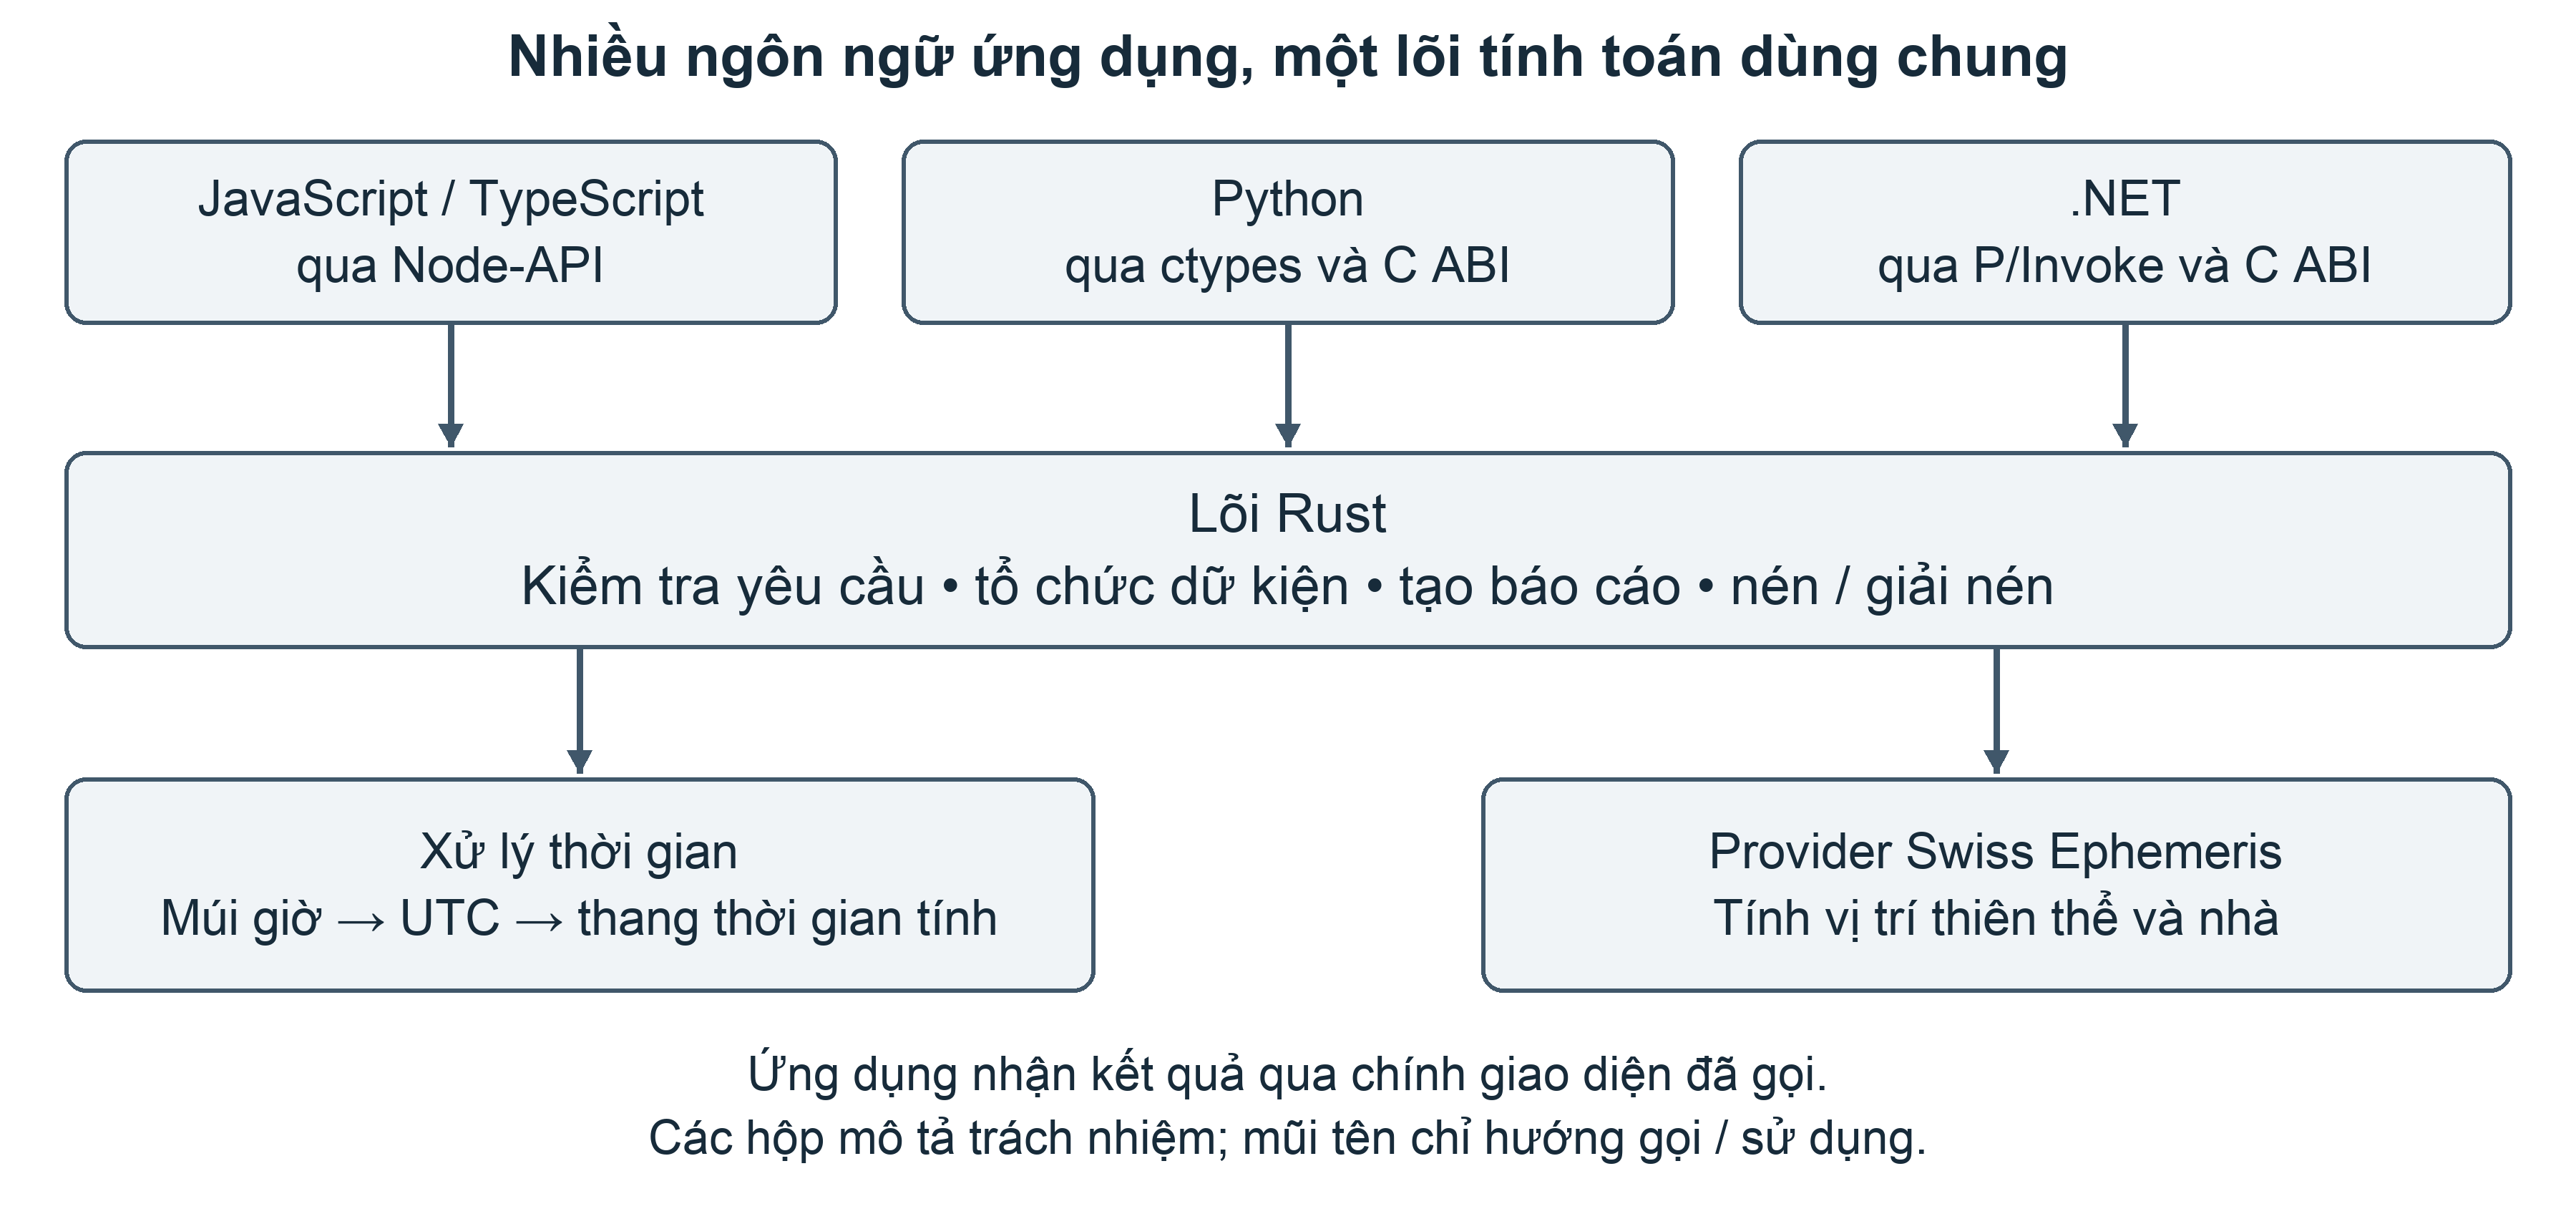
\includegraphics[width=\linewidth]{images/01-kien-truc.png}
\par\smallskip\raggedright{\fontsize{10}{12}\selectfont\itshape Hình 1. Các lớp kiến trúc chính của Astro SDK. Mũi tên là hướng gọi hoặc sử dụng, không phải số đo tốc độ. Sơ đồ biên soạn từ mã và tài liệu dự án [1, 7, 8].\par}\end{minipage}\par\medskip
\section*{3 Phương pháp và phạm vi bằng chứng}
\subsection*{3.1 Phiên bản và dữ liệu được kiểm tra}
Nghiên cứu dùng mã sản phẩm tại commit cd768d0192cd, phiên bản 1.0.0 khai báo trong dự án; mã commit đầy đủ ở phụ lục A. Mã sản phẩm không được sửa. Phần đọc sâu gồm thư viện thiên văn, xử lý thời gian, giao diện C và bộ nén; các mô-đun khác được bao phủ ở mức các kiểm thử hiện có, không được tuyên bố đã đánh giá chuyên sâu từng thuật toán. [1, 7, 8]


Bộ đo nén gồm toàn bộ 17 tệp examples/\allowbreak{}*-result.json có tại phiên bản mã này, chọn trước phép đo đầu tiên. Cả 17 gói nguồn mang engineVersion 0.10.0-alpha.1. Vì vậy đây là kiểm tra bộ nén 1.0.0 trên mẫu lịch sử, không phải khảo sát toàn bộ đầu ra mới của SDK 1.0.0. Mẫu do dự án cung cấp, không lấy ngẫu nhiên từ người sử dụng. Không loại tệp dựa trên mức giảm kích thước. [9]


Đề cương được lập sau lượt đọc tài liệu ban đầu. Lượt rà soát 1.1 giữ nguyên bộ mẫu nhưng làm chặt công cụ so sánh và bổ sung dữ liệu thô. Đây là điều chỉnh phương pháp được công bố sau khi đã biết kết quả ban đầu, không phải đăng ký trước nghiên cứu hay một phép lặp độc lập do nhóm khác thực hiện. [9]


\subsection*{3.2 Kiểm tra bảo toàn thông tin}
Mỗi tệp nguồn được truyền nguyên văn đến chương trình dòng lệnh Rust để nén compact, rồi đầu ra native được truyền nguyên văn vào bước giải nén. Cách này tránh một lượt đổi số qua bộ đọc/\allowbreak{}ghi của Python trước khi native nhận dữ liệu. Bộ kiểm tra đọc nguồn và kết quả giải nén bằng số thập phân Decimal, sau đó đối chiếu đệ quy từng phần tử. [9]


Quy tắc là: giữ cùng tên trường, cấu trúc, thứ tự mảng, chuỗi, giá trị số và các giá trị true, false, null. true không được coi bằng số 1, false không được coi bằng số 0. Thứ tự tên trường và khoảng trắng không cần giống; 1 và 1.0 được xem là cùng giá trị số. Ví dụ, đổi null thành false là mất thông tin, còn viết 0.000001 thành 1e-6 chỉ thay cách ghi cùng một số. Quy tắc phân biệt kiểu bám theo các loại giá trị JSON; cách so sánh số tương đương là lựa chọn được công bố của nghiên cứu. [9, 11]


Trước khi kiểm tra 17 mẫu, công cụ so sánh được thử bằng các trường hợp cố ý đổi kiểu, đổi số, đảo mảng và bỏ trường, cùng các trường hợp tương đương hợp lệ. Công cụ còn từ chối tên trường trùng và hằng số không hợp lệ NaN/\allowbreak{}Infinity. Việc từ chối tên trường trùng là quy tắc của bộ đo; RFC 8259 khuyến nghị tên trường duy nhất, không cấm cú pháp trùng tên trong mọi bộ đọc JSON. [11] Các kiểm tra công cụ này không được cộng vào số kiểm thử của sản phẩm. Chúng kiểm tra bộ đo, không chứng minh khả năng bảo toàn mọi JSON có thể có. [9]


\subsection*{3.3 Vì sao khôi phục đúng đòi hỏi giữ được sự khác biệt}
Hãy hình dung hai hồ sơ chỉ khác nhau ở một trường thông tin. Nếu sau khi nén chúng trở thành cùng một gói dữ liệu, bên giải nén chỉ nhìn thấy một đầu vào và không biết phải khôi phục hồ sơ nào. Trực giác này dẫn đến một điều kiện cần cho mọi cách nén có thể khôi phục đầy đủ, không riêng Astro.


Xét miền X gồm các gói JSON không có tên trường trùng, với quy tắc so sánh ở mục 3.2. Gọi x là một gói thuộc X, E là phép nén compact và D là phép giải nén xác định: cùng một đầu vào thì D cho cùng một kết quả. Giả sử E tạo được biểu diễn cho mọi x trong X và D trả về dữ liệu khi nhận các biểu diễn đó. Ký hiệu \(\equiv\) nghĩa là tương đương theo cấu trúc, kiểu và giá trị đã định nghĩa ở mục 3.2, không yêu cầu văn bản giống từng ký tự. E(x) bao gồm toàn bộ context và thông tin cần để giải mã; bộ giải mã và phiên bản định dạng được giữ cố định. Điều kiện khôi phục mong muốn là:


\begin{equation}D(E(x))\equiv x\qquad\text{với mọi }x\in X.\label{eq:ROUNDTRIP}\end{equation}
Mệnh đề 1 — điều kiện cần. Nếu (1) đúng cho mọi đầu vào trong X, hai đầu vào không tương đương không thể cho cùng một biểu diễn nén. Ở đây “cùng biểu diễn nén” nghĩa là bên giải nén nhận đúng cùng một đầu vào, không có thông tin phụ để phân biệt.


Chứng minh. Giả sử ngược lại có x và y không tương đương nhưng E(x) = E(y). Vì D xác định, giải nén hai biểu diễn giống nhau cho cùng một kết quả. Áp dụng (1) cho cả x và y cho chuỗi suy luận sau:


\begin{equation}x\equiv D(E(x))=D(E(y))\equiv y.\label{eq:INJECTIVE}\end{equation}
Quan hệ \(\equiv\) có tính đối xứng và bắc cầu theo quy tắc so sánh đã chọn, nên chuỗi (2) suy ra x \(\equiv\) y. Kết luận này trái với giả sử ban đầu; vì vậy hai biểu diễn nén phải khác nhau. Đây là chứng minh điều kiện cần, không phải chứng minh rằng một cài đặt cụ thể đã thỏa (1). Nó cũng không chứng minh rằng kích thước sau nén sẽ nhỏ hơn.


Ví dụ, hai gói có trường ghiChu lần lượt là “A” và “B”. Nếu phép biến đổi xóa trường đó và không lưu giá trị ở nơi khác, phần còn lại có thể giống hệt nhau. Bộ giải mã không thể khôi phục đúng cả hai gói. Điều này giải thích vì sao bỏ dữ liệu theo phạm vi cần được phân biệt với đổi cách biểu diễn dữ liệu. Đối với triển khai Astro, đầu vào nén phải là gói phản hồi chuẩn của engine và chịu giới hạn kích thước, độ sâu; không phải JSON bất kỳ đều được chấp nhận. Với Astro, focused và budgeted công bố phần bị bỏ; bài không áp dụng cam kết khôi phục toàn bộ nguồn cho hai chế độ đó. [8]


Bằng chứng thực nghiệm của bài chỉ kiểm tra (1) trên tập S gồm 17 mẫu đã chọn: mỗi mẫu được nén, giải nén và so sánh đầy đủ bằng công cụ ở mục 3.2. Mệnh đề được chứng minh ở trên áp dụng theo giả thiết của nó; kết quả 17/\allowbreak{}17 không cho phép thay S bằng toàn bộ JSON. Đây là ranh giới giữa lập luận toán học và bằng chứng về phần mềm. [9]


\subsection*{3.4 Công thức đo dung lượng và cách suy dẫn}
Câu hỏi tiếp theo là: khi dữ liệu khôi phục đúng, ta đã giảm được bao nhiêu dung lượng? Trước hết phải chọn cùng một mốc so sánh. Mốc của bài là số byte UTF-8 của toàn bộ gói nguồn sau khi lõi Rust viết lại ở dạng gọn. Kích thước sau nén bao gồm cả dữ liệu, bảng tham chiếu, thông tin phạm vi, phiên bản và cảnh báo. outputBytes được đối chiếu với byte đầu ra native thực tế; inputBytes được đối chiếu với byte của gói giải nén native sau khi đã xác nhận cùng giá trị với nguồn. Hai phép đếm đều bỏ ký tự xuống dòng do chương trình dòng lệnh thêm. [8, 9]


Trực giác. Nếu một gói từ 100 byte còn 60 byte thì đã bớt 40 byte, tức 40 phần trong mỗi 100 phần ban đầu. Với kích thước bất kỳ, gọi B > 0 là byte nguồn, C ≥ 0 là byte sau nén và ΔB là số byte giảm. R là con số phần trăm giảm; chẳng hạn R = 40 được đọc là giảm 40\%. Ta có:


\begin{equation}\Delta B=B-C,\qquad R=100\frac{B-C}{B}=100\left(1-\frac{C}{B}\right).\label{eq:REDUCTION}\end{equation}
Suy dẫn. Lấy B − C để đếm số byte đã bớt; chia cho B để tính phần đã bớt so với ban đầu; nhân 100 để biểu diễn theo phần trăm. Tách phân số cho dạng tương đương 100(1 − C/\allowbreak{}B). Vì B > 0, dấu của R chính là dấu của B − C: R > 0 là nhỏ hơn, R = 0 là không đổi, R < 0 là lớn hơn. Vì C ≥ 0 nên R ≤ 100; không có cận dưới chung nếu C/\allowbreak{}B có thể tăng không giới hạn. Đây là hệ quả đại số của định nghĩa, không phải cam kết hiệu quả của bộ nén.


Với số đo tổng của 17 mẫu, B = 20.014.085 byte và C = 11.554.591 byte, phép trừ cho 8.459.494 byte. Chia phần đã giảm cho B rồi nhân 100 được khoảng 42,27\%. Phần còn lại là 100C/\allowbreak{}B ≈ 57,73\%; hai phần cộng thành 100\%. Hình 2 minh họa phép tính này. [9]


\par\medskip\noindent\begin{minipage}{\linewidth}\centering
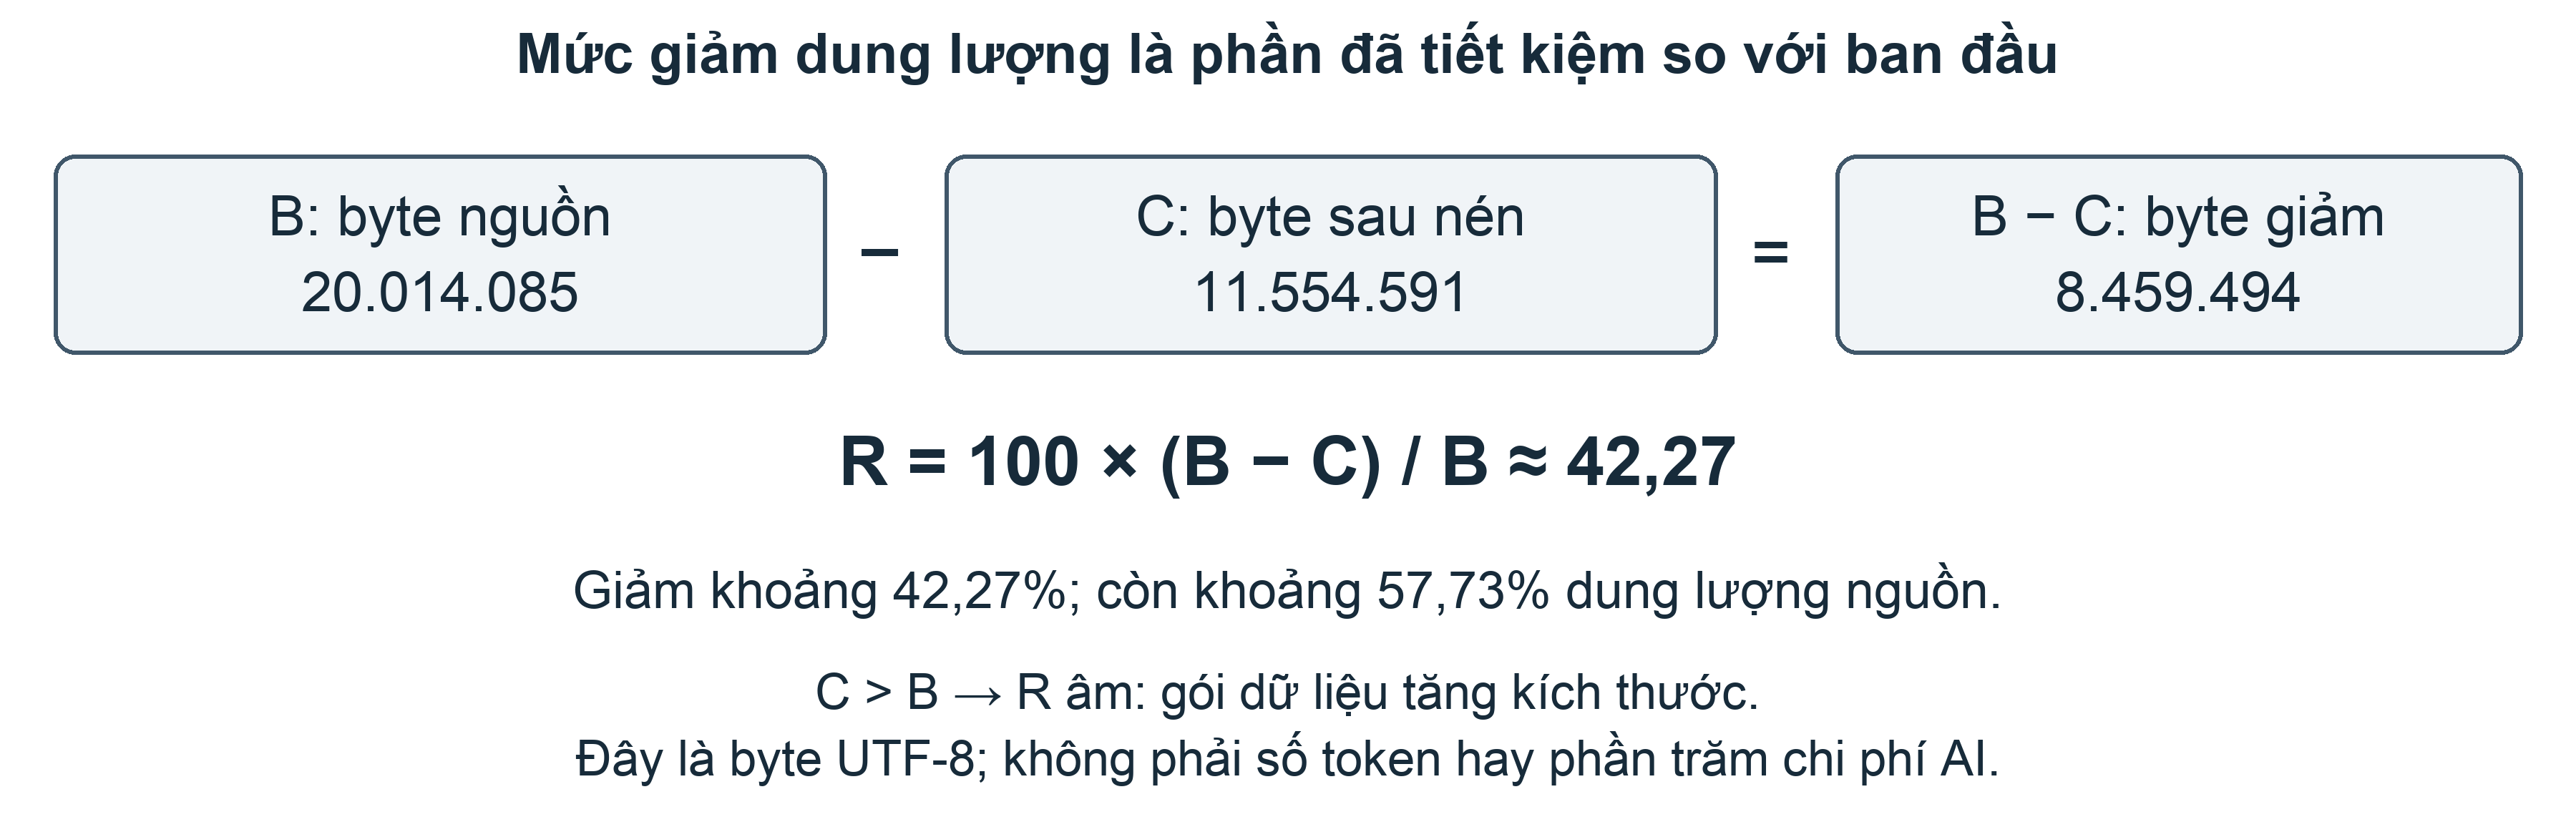
\includegraphics[width=\linewidth]{images/03-cong-thuc.png}
\par\smallskip\raggedright{\fontsize{10}{12}\selectfont\itshape Hình 2. Minh họa công thức (3) bằng tổng byte đo được của 17 mẫu. Nguồn số đo: [9]. Hình và phép suy dẫn do nghiên cứu biên soạn; byte không phải token hoặc chi phí AI.\par}\end{minipage}\par\medskip
Mệnh đề 2 — mức giảm tổng là trung bình có trọng số theo byte nguồn. Với n là số nguyên dương, các gói được đánh số từ 1 đến n. \(B_{i}\) > 0 và \(C_{i}\) ≥ 0 lần lượt là số byte trước và sau nén của gói i. \(R_{i}\) là mức giảm của gói đó theo (3). Đặt \(w_{i}\) = \(B_{i}\) /\allowbreak{} tổng \(B_{j}\), tức tỷ phần dung lượng nguồn do gói i đóng góp. Ký hiệu Σ là phép cộng qua các gói; i và j chỉ là chỉ số chạy từ 1 đến n. Khi đó:


\begin{equation}R_{\text{tổng}}=100\frac{\sum_{i=1}^{n}(B_i-C_i)}{\sum_{i=1}^{n}B_i}=\sum_{i=1}^{n}w_iR_i,\qquad w_i=\frac{B_i}{\sum_{j=1}^{n}B_j}.\label{eq:WEIGHTED}\end{equation}
Chứng minh. Thay định nghĩa \(R_{i}\) vào tổng có trọng số; \(B_{i}\) ở tử và mẫu của mỗi số hạng triệt tiêu. Các số hạng còn lại dùng chung mẫu là tổng byte nguồn, nên cộng các tử số cho đúng mức giảm tổng:


\begin{equation}\sum_{i=1}^{n}w_iR_i=\sum_{i=1}^{n}\frac{B_i}{\sum_{j=1}^{n}B_j}\,100\frac{B_i-C_i}{B_i}=100\frac{\sum_{i=1}^{n}(B_i-C_i)}{\sum_{j=1}^{n}B_j}.\label{eq:WEIGHTED_PROOF}\end{equation}
Các trọng số \(w_{i}\) dương và cộng bằng 1 vì tổng tử số bằng mẫu số. Mỗi \(R_{i}\) nằm giữa mức nhỏ nhất và lớn nhất; nhân từng bất đẳng thức với \(w_{i}\) rồi cộng lại cho thấy mức giảm tổng cũng nằm trong hai mức đó. Tuy nhiên nó không phải trung bình cộng thông thường của \(R_{i}\): gói lớn có ảnh hưởng nhiều hơn. Ví dụ minh họa, không phải số đo Astro: một gói 900 byte giảm 50\%, một gói 100 byte giảm 0\%; tổng giảm 450/\allowbreak{}1.000 = 45\%, trong khi trung bình cộng hai tỷ lệ chỉ là 25\%.


Trong dữ liệu Astro, tổng giảm 42,27\% và trung vị là 40,12\%. Trung vị là tỷ lệ đứng thứ 9 sau khi xếp 17 tỷ lệ từ nhỏ đến lớn; nó không dùng trọng số byte. Hai con số trả lời hai câu hỏi khác nhau: “toàn bộ lô giảm bao nhiêu?” và “mẫu ở giữa giảm bao nhiêu?”. Không con số nào tự dự báo mức giảm cho người dùng mới. Mỗi mẫu được chạy một chu trình trong lượt rà soát; bài không đo độ trễ, bộ nhớ hoặc token của một mô hình cụ thể. [9]


\subsection*{3.5 Vì sao sai lệch kinh độ phải đo trên vòng tròn}
Kinh độ là một góc trên vòng tròn: 0° và 360° chỉ cùng một hướng. Vì vậy, hai vị trí 359° và 1° nằm gần nhau qua mốc 0°; lấy hiệu tuyệt đối thông thường sẽ cho 358° và dễ gây hiểu nhầm. Ta cần độ dài góc của cung ngắn hơn.


Gọi a và b là hai kinh độ hữu hạn của cùng thiên thể, cùng đơn vị độ, cùng thời điểm và quy ước tọa độ. Đặt δ là phần dư không âm khi chia |a − b| cho 360°, nên 0° ≤ δ < 360°. Độ lệch góc d được tính như sau:


\begin{equation}\delta=|a-b|\bmod 360^\circ,\qquad d(a,b)=\min\!\left(\delta,360^\circ-\delta\right).\label{eq:ANGLE}\end{equation}
Chứng minh. Hai cung nối hai hướng trên một vòng tròn có góc δ và 360° − δ, tổng bằng một vòng. Đi thêm một hoặc nhiều vòng chỉ làm đường đi dài hơn. Do đó góc nhỏ nhất là giá trị nhỏ hơn của hai cung, nằm trong khoảng 0° đến 180°. Với a = 359° và b = 1°, δ = 358° nên d = min(358°, 2°) = 2°. Hai hướng trùng nhau cho d = 0°; hai hướng đối nhau cho d = 180°. Đây là tính chất hình học của phép đo, không chứng minh các tọa độ đầu vào đã chính xác. Công thức chỉ đo chênh lệch kinh độ; khoảng cách góc đầy đủ giữa hai vị trí trên thiên cầu còn phụ thuộc vĩ độ thiên thể.


Mã phân tích áp dụng đúng phép lấy phần dư và lấy giá trị nhỏ hơn này khi so kinh độ Astro với tham chiếu. [9] Điều kiện cùng hệ quy chiếu và cách hiệu chỉnh vị trí cần được giữ trước khi so sánh; tài liệu Skyfield giải thích các loại vị trí khác nhau. [3] Bài tính lại bốn yêu cầu lá số trong fixture, mỗi yêu cầu có mười thiên thể. Hai yêu cầu cùng thời điểm năm 2000 nhưng khác hệ nhà, nên chỉ có ba thời điểm thiên văn riêng biệt. Chỉ kinh độ được đo lại; không suy rộng sang mọi tọa độ, vận tốc, điểm mở rộng hoặc thời điểm sự kiện. [4, 9]


Một độ gồm 60 phút cung, mỗi phút cung gồm 60 giây cung; vì thế nhân số độ với 3.600 để đổi sang giây cung. Sai lệch lớn nhất với Skyfield lưu sẵn, khoảng 0,0001213184°, tương ứng khoảng 0,437 giây cung. Đơn vị này đo góc, không đo thời gian. Số liệu và giới hạn đối chiếu được trình bày ở mục 5.3. [4, 9]


\subsection*{3.6 Môi trường và cách đọc mức độ bằng chứng}
Bộ kiểm thử Rust được chạy lại bằng tệp khóa phiên bản thư viện trên macOS 26.1 ARM64, rustc/\allowbreak{}cargo 1.93.1. Chương trình dòng lệnh (CLI) dùng cấu hình biên dịch dev. Thời gian hoàn tất kiểm thử không được dùng làm thước đo hiệu năng. Các số đo ở mục 5 thuộc lượt rà soát 1.1; các bản 1.3–1.4 bổ sung suy dẫn, rà soát và cách trình bày, không bổ sung một lượt thực nghiệm sản phẩm mới. [9, 10]


Cách đọc các bằng chứng là: công thức định nghĩa điều cần đo; chứng minh chỉ ra hệ quả của giả thiết; mã và log cho biết phép đo đã được thực hiện ra sao; kết quả hữu hạn xác định phạm vi kết luận. Các công thức ở đây giải thích phép kiểm tra dữ liệu và phép so góc. Bài không suy dẫn lại mô hình chuyển động thiên thể bên trong Swiss Ephemeris, và không coi các chứng minh này là chứng nhận toàn bộ SDK.


\section*{4 Kết quả phân tích chuỗi xử lý}
\subsection*{4.1 Các bước từ đầu vào đến gói kết quả}
Hình 3 minh họa một yêu cầu natal, tức tính lá số tại một thời điểm và địa điểm. Đọc hàng trên từ trái sang phải, sau đó đi xuống và đọc hàng dưới từ phải sang trái. Bước chọn cách chuyển dữ liệu là tùy chọn của bên sử dụng; việc nén không phải điều kiện bắt buộc để nhận kết quả. Bảng 1 bổ sung trách nhiệm cần kiểm tra ở từng ranh giới. [1, 7, 8]


\par\medskip\noindent\begin{minipage}{\linewidth}\centering
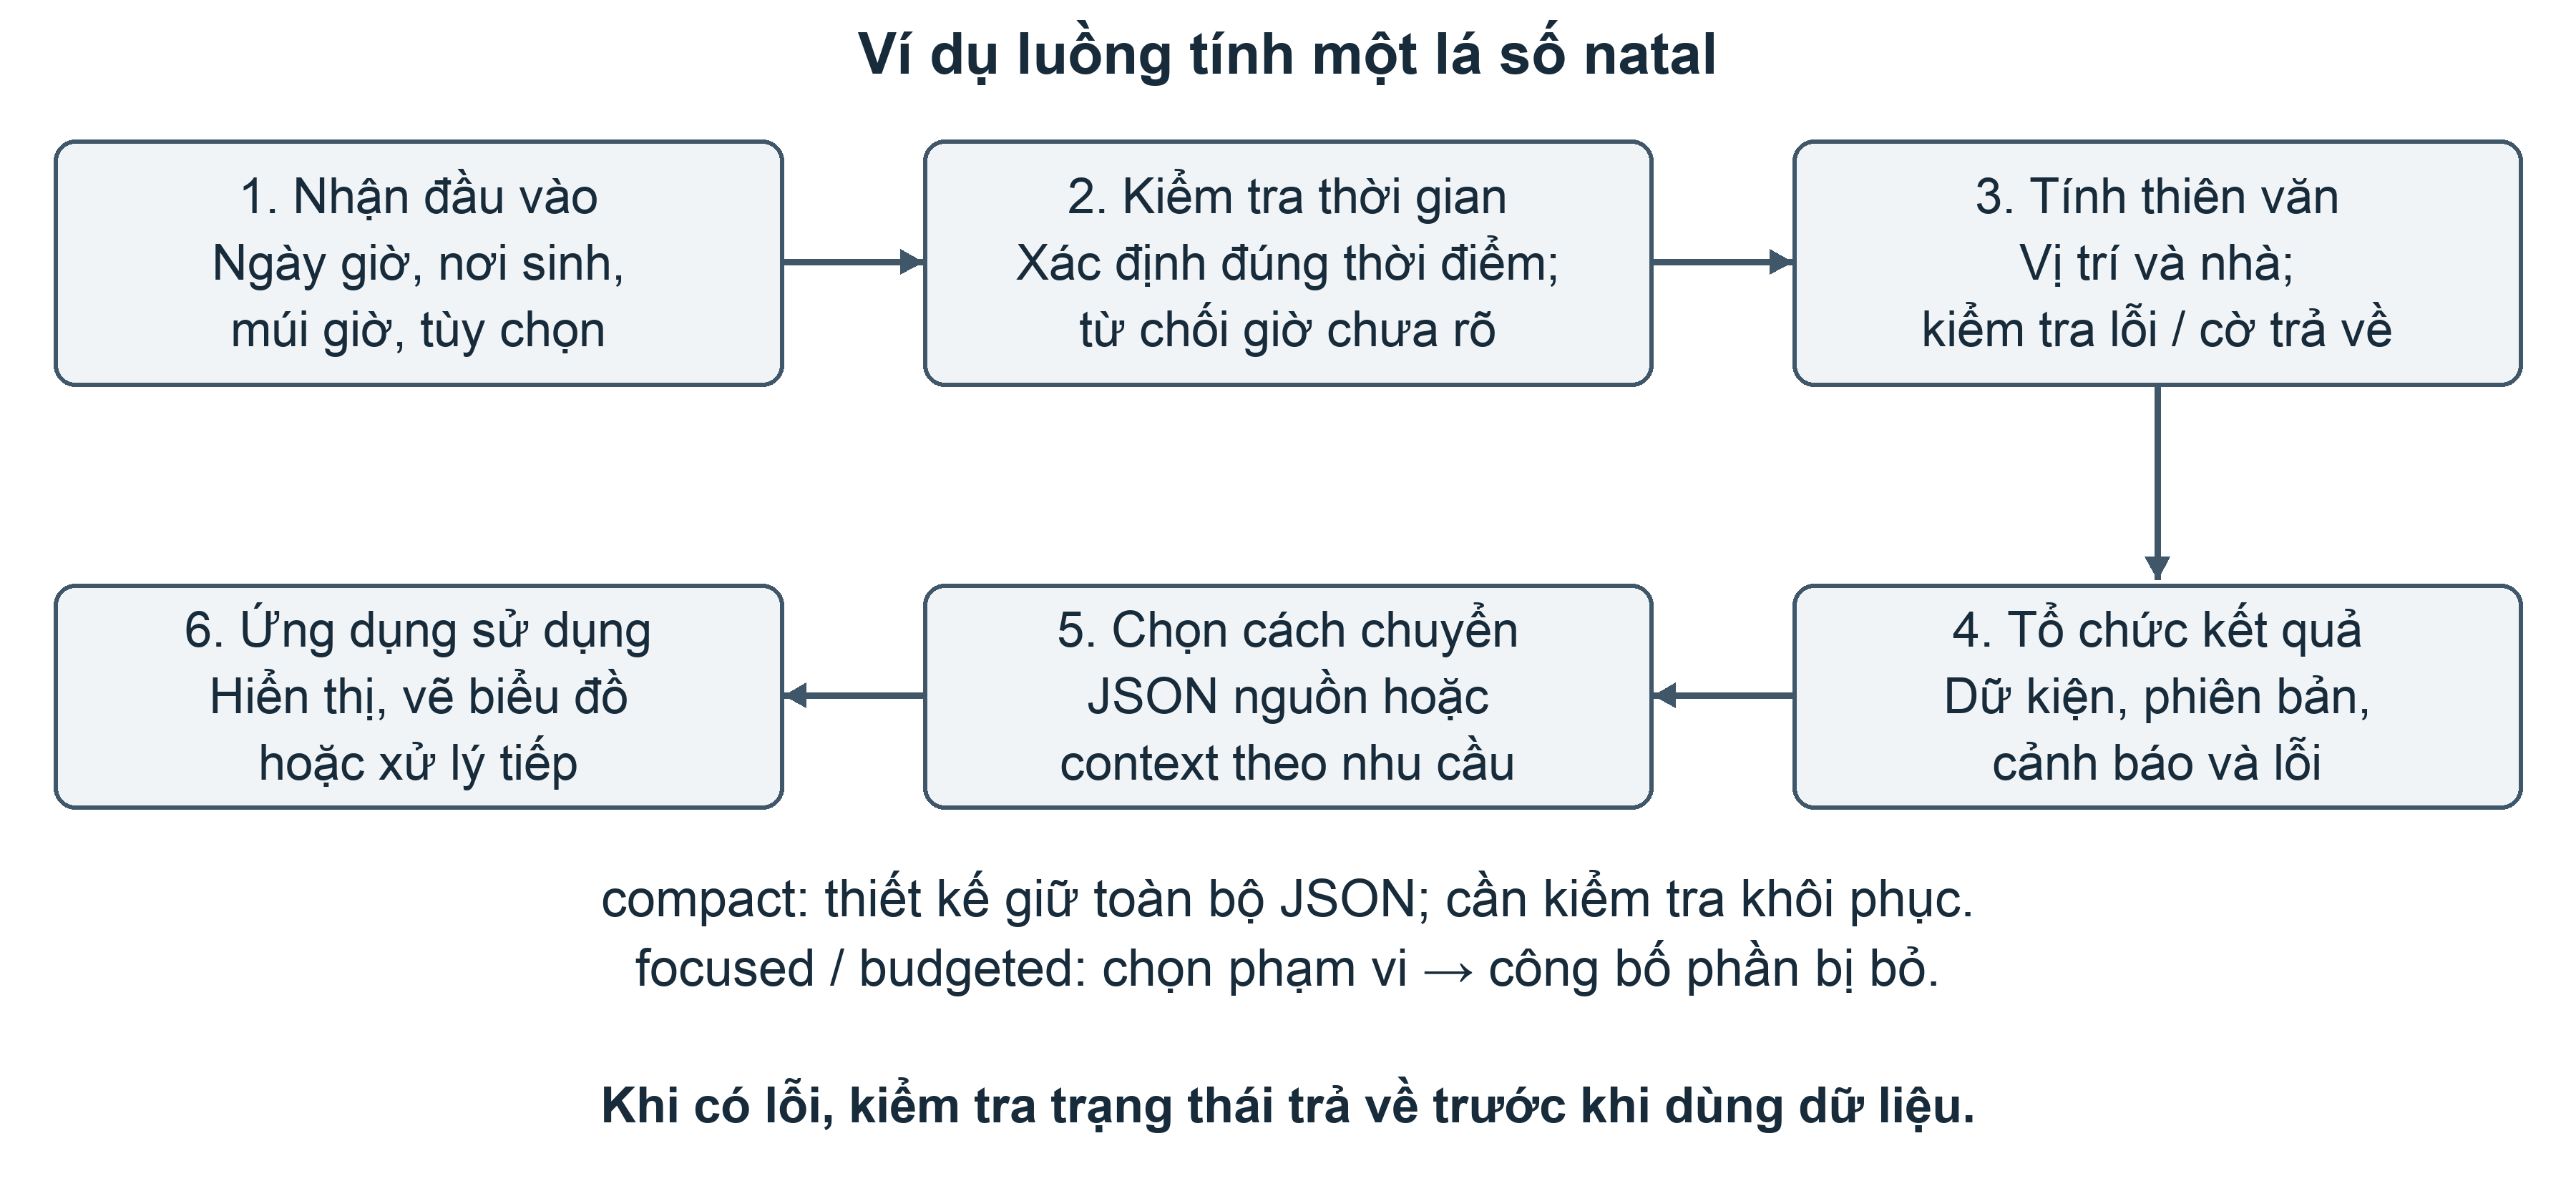
\includegraphics[width=\linewidth]{images/02-luong-xu-ly.png}
\par\smallskip\raggedright{\fontsize{10}{12}\selectfont\itshape Hình 3. Luồng khái quát từ yêu cầu natal đến ứng dụng sử dụng kết quả. Nhánh lỗi được tóm tắt bằng điều kiện kiểm tra trạng thái; sơ đồ không biểu diễn mọi nhánh trong mã. Nguồn: [1, 7, 8].\par}\end{minipage}\par\medskip
Bảng 1 trình bày luồng xử lý ở mức người sử dụng. “Hợp đồng” trong bài nghĩa là điều kiện mà đầu vào, đầu ra hoặc bên gọi phải đáp ứng. Bảng mô tả triển khai và trách nhiệm, không phải kết quả đo hiệu năng. [1, 7, 8]


\Needspace{6\baselineskip}\par\medskip\noindent{\fontsize{10}{12}\selectfont\itshape Bảng 1. Chuỗi xử lý và ý nghĩa của từng ranh giới. Nguồn: mã và tài liệu dự án [1, 7, 8].\par}\nopagebreak
{\fontsize{10}{12}\selectfont\begin{longtable}{>{\raggedright\arraybackslash}p{\dimexpr 0.21\linewidth-2\tabcolsep\relax}>{\raggedright\arraybackslash}p{\dimexpr 0.39\linewidth-2\tabcolsep\relax}>{\raggedright\arraybackslash}p{\dimexpr 0.4\linewidth-2\tabcolsep\relax}}
\toprule \textbf{Bước} & \textbf{Công việc của SDK} & \textbf{Điều vẫn cần kiểm tra} \\ \midrule
\endfirsthead\toprule \textbf{Bước} & \textbf{Công việc của SDK} & \textbf{Điều vẫn cần kiểm tra} \\ \midrule\endhead\bottomrule\endfoot

Giờ địa phương & Chọn múi giờ hoặc độ lệch để đổi sang UTC & Giờ ghi nhận ban đầu và lựa chọn khi giờ xuất hiện hai lần \\
Phép tính thiên văn & Dùng Swiss Ephemeris, kiểm tra mô hình và lỗi trả về & Phạm vi ngày, quy ước tọa độ và độ chính xác theo mục đích \\
Tổ chức dữ kiện & Tạo biểu đồ, quan hệ và báo cáo theo quy tắc & Cơ sở của quy tắc diễn giải; không suy từ việc có dữ kiện \\
Chuyển qua ngôn ngữ & Các giao diện gọi lõi Rust dùng chung & Cài đặt gói, chuyển kiểu và bộ nhớ trên từng nền tảng \\
Chuẩn bị context & Giữ toàn bộ hoặc chọn phạm vi, công bố phần bỏ & Dữ liệu còn lại có đủ cho câu hỏi và phía nhận hay không \\
\end{longtable}}
Một lõi chung giúp nhiều giao diện dùng cùng công thức. Tuy nhiên wrapper, tức lớp nối giữa ngôn ngữ ứng dụng và lõi native, vẫn có thể sai khi chuyển kiểu hoặc quản lý bộ nhớ. Do đó kiến trúc dùng chung và đầu ra giống nhau trên mọi gói là hai vấn đề khác nhau: vấn đề thứ hai cần phép thử trên chính các gói đó. [1, 7]


\subsection*{4.2 Thời gian và lỗi không được sửa ngầm}
Ở bước đổi giờ, astro-time yêu cầu tên múi giờ IANA hoặc độ lệch UTC được chỉ định. Giờ không tồn tại trong một lần chuyển giờ mùa hè bị từ chối. Khi một giờ xuất hiện hai lần, mặc định cũng từ chối cho tới khi bên gọi chọn lần sớm hơn hoặc muộn hơn. Trong bộ kiểm thử đã chạy, giờ 01:30 tại New York ngày 03/\allowbreak{}11/\allowbreak{}2024 được kiểm tra với hai lựa chọn có giờ UTC lần lượt là 05 và 06; ca giờ không tồn tại ngày 10/\allowbreak{}03/\allowbreak{}2024 bị từ chối. [7, 9]


Ý nghĩa thực tế là ứng dụng phải hỏi lại hoặc dùng hồ sơ đáng tin cậy để giải quyết sự mơ hồ. Tự chọn một nhánh không làm dữ liệu gốc trở nên đúng hơn. Mã cũng cảnh báo về dữ liệu lịch sử trước năm 1970 và quy tắc múi giờ tương lai. Giới hạn nhận năm 1800–2399 là giới hạn đầu vào, không phải cam kết mọi hồ sơ thời gian trong khoảng đó đều chính xác. [7]


\subsection*{4.3 Trạng thái thư viện và giao diện native}
Provider, tức lớp gọi thư viện thiên văn, dùng khóa Mutex trong từng thư viện native. Có thể hiểu khóa như quyền sử dụng độc quyền một vùng trạng thái dùng chung: một phép tính phải hoàn tất phần được bảo vệ trước khi phép tính khác vào đó. Lời gọi natal giữ khóa qua các bước khởi tạo, chuyển đổi thời gian, tính vị trí, nhà và dọn trạng thái; phiên quét giữ khóa trong thời gian phiên tồn tại. Điều này kiểm soát truy cập trạng thái nhưng có thể hạn chế xử lý đồng thời. Nghiên cứu chưa đo mức hạn chế đó. [7]


Trong nhánh natal của mười thiên thể cơ bản, mã kiểm tra vị trí trả về là số hữu hạn và đúng cờ Moshier, mô hình đã chọn. Khi hệ nhà được yêu cầu không tính được, mã trả lỗi, không công bố kết quả dự phòng như một kết quả đúng yêu cầu. Đây là quan sát nhánh xử lý trong mã; bài không báo đã thực hiện một chiến dịch chèn lỗi mới. Hai hệ nhà Placidus và Whole Sign là hai quy tắc chia vùng trên biểu đồ, không phải hai mô hình chuyển động hành tinh. [7]


Giao diện C yêu cầu chuỗi kết quả do Rust cấp phát phải được giải phóng đúng một lần bằng hàm của Rust. Mã xử lý con trỏ null, dữ liệu không phải UTF-8 và panic Rust theo các nhánh đã định nghĩa. Tuy nhiên bên gọi vẫn phải cung cấp con trỏ hợp lệ; cơ chế bắt panic không bảo vệ trước mọi lỗi địa chỉ bộ nhớ. Sự an toàn của giao diện còn phụ thuộc bên gọi tuân thủ hợp đồng này. [7]


“Chạy offline” ở đây không đồng nghĩa không có dữ liệu thiên văn đi kèm. Nhánh hành tinh cơ bản dùng Moshier và chặn việc đọc dữ liệu ngoài; riêng dữ liệu cho Chiron được nhúng trong binary theo hồ sơ nguồn gốc. Đây là mô tả thiết kế và hồ sơ nguồn gốc đã đọc, không phải kết quả một cuộc kiểm tra lưu lượng mạng của mọi ứng dụng dùng SDK. [7]


\subsection*{4.4 Ba chế độ rút gọn có cam kết khác nhau}
compact được thiết kế để đổi cách biểu diễn mà giữ toàn bộ gói kết quả ở mức giá trị JSON. Khả năng khôi phục được kiểm tra trên 17 mẫu ở mục 5.2, chưa được chứng minh cho mọi đầu vào mà triển khai nhận. Có thể hình dung các tên cột được viết một lần thay vì lặp lại ở mỗi dòng, còn dữ liệu giống nhau được dùng qua bảng tham chiếu. focused chỉ giữ những lĩnh vực hoặc phần báo cáo được chọn. budgeted thêm kiểm tra giới hạn kích thước; nếu vẫn quá lớn thì báo vượt, không tự cắt thêm dữ kiện chỉ để đạt giới hạn. [8]


Khi có phần bị bỏ trong các chế độ chọn phạm vi, trường omitted liệt kê phần đó; giải nén không tái tạo được thông tin đã bỏ. Nếu không bỏ phần nào, cần đọc coverage.complete và omitted để xác định phạm vi thực tế, thay vì chỉ nhìn tên chế độ. Việc giữ các cấu trúc chia sẻ tránh làm đổi nghĩa các chỉ mục tham chiếu, nhưng có thể làm mức giảm kích thước hạn chế. Bài chỉ đo compact trên toàn bộ 17 mẫu; không lấy kết quả này làm tỷ lệ nén của focused hoặc budgeted. [8, 9]


Trường estimatedTokens hiện lấy giá trị từ số byte UTF-8. Nó chưa phải số token do bộ tách từ của một mô hình AI tính ra. Vì thế “giảm 42,27\% byte” không đồng nghĩa “giảm 42,27\% hóa đơn AI”, và khả năng giải nén đúng cũng chưa chứng minh mô hình sẽ đọc đúng biểu diễn đã nén. [8]


\section*{5 Kết quả thực thi và cách diễn giải}
\subsection*{5.1 Bộ kiểm thử sản phẩm}
Lượt chạy lại hoàn tất với 132 kiểm thử đạt, không có ca thất bại hoặc bị bỏ qua trong các nhóm đã chạy. Các ca này gồm kiểm thử lõi, hợp đồng báo cáo, thư viện thiên văn, thời gian, giao diện C và bộ vẽ SVG. Phụ lục A ghi số ca theo nhóm để kiểm tra lại tổng; không cộng các nhóm doc-test không có ca thử. [9]


Con số 132 có nghĩa phần mềm cho kết quả như các điều kiện đã viết trong bộ test. Nó không có nghĩa đã kiểm tra 132 người dùng, toàn bộ đầu vào hoặc mọi nền tảng. Tài liệu phát hành báo cáo 339 trường hợp đối chiếu giữa các binding; ma trận đó không được chạy lại trong nghiên cứu này và không được cộng với 132 để tạo một tổng “độ tin cậy”. [9, 10]


\subsection*{5.2 Khôi phục dữ liệu và mức giảm kích thước}
Cả 17 mẫu vượt qua phép so sánh cấu trúc, kiểu và giá trị JSON đã mô tả. Trong cả 17 trường hợp, dữ liệu phạm vi báo đầy đủ, danh sách bỏ trống, byte đầu ra và byte nguồn native được đối chiếu đúng theo mục 3.4. Kết quả chỉ áp dụng các mẫu này; nghiên cứu không vét cạn mọi giá trị số hoặc cấu trúc JSON. [9]


Theo mốc nguồn native ở mục 3.4, tổng nguồn là 20.014.085 byte; tổng context là 11.554.591 byte, giảm 8.459.494 byte hay 42,27\%. Có 15 mẫu giảm và hai mẫu tăng kích thước. Trung vị mức giảm theo mẫu là 40,12\%; khoảng quan sát từ −43,11\% đến 51,03\%. Đây là thống kê mô tả của bộ mẫu có sẵn, không phải khoảng tin cậy hoặc mức tiết kiệm bảo đảm. [9]


\Needspace{6\baselineskip}\par\medskip\noindent{\fontsize{10}{12}\selectfont\itshape Bảng 2. Nén compact trên cả 17 mẫu. Tên tệp bỏ hậu tố -result.json. R là mức giảm phần trăm; R âm là tăng kích thước. Nguồn: lượt chạy rà soát [9].\par}\nopagebreak
{\fontsize{10}{12}\selectfont\begin{longtable}{>{\raggedright\arraybackslash}p{\dimexpr 0.37\linewidth-2\tabcolsep\relax}>{\raggedleft\arraybackslash}p{\dimexpr 0.22\linewidth-2\tabcolsep\relax}>{\raggedleft\arraybackslash}p{\dimexpr 0.22\linewidth-2\tabcolsep\relax}>{\raggedleft\arraybackslash}p{\dimexpr 0.19\linewidth-2\tabcolsep\relax}}
\toprule \textbf{Mẫu} & \textbf{Nguồn byte} & \textbf{Context byte} & \textbf{R \%} \\ \midrule
\endfirsthead\toprule \textbf{Mẫu} & \textbf{Nguồn byte} & \textbf{Context byte} & \textbf{R \%} \\ \midrule\endhead\bottomrule\endfoot

composite & 2.206.657 & 1.374.846 & 37,70 \\
couple-composite & 4.126.966 & 2.353.132 & 42,98 \\
couple & 2.101.342 & 1.101.529 & 47,58 \\
custom-composite & 319.866 & 191.531 & 40,12 \\
custom-couple & 709.819 & 386.109 & 45,60 \\
custom-forecast & 411.884 & 201.689 & 51,03 \\
custom-profiles & 256.206 & 143.847 & 43,85 \\
events-year & 1.264.416 & 1.054.977 & 16,56 \\
forecast-day & 306.138 & 158.573 & 48,20 \\
forecast-month & 4.296.721 & 2.195.074 & 48,91 \\
forecast-year & 1.828.614 & 1.062.147 & 41,92 \\
natal-domains & 2.129.952 & 1.291.076 & 39,38 \\
natal & 7.147 & 5.269 & 26,28 \\
query-aspects & 1.908 & 2.266 & -18,76 \\
query-between & 900 & 1.288 & -43,11 \\
query-houses & 28.666 & 18.636 & 34,99 \\
query-points & 16.883 & 12.602 & 25,36 \\
\end{longtable}}
Ví dụ, query-between từ 900 lên 1.288 byte: tăng 388 byte, tức 43,11\%. query-aspects tăng 358 byte, tức 18,76\%. Phần thông tin bổ sung và biểu diễn của context có thể lớn hơn lượng lặp được loại bỏ ở gói nhỏ. Hai mẫu này đủ bác bỏ nhận định “compact luôn làm nhỏ dữ liệu”. Chúng không chứng minh mọi gói nhỏ đều tăng kích thước hoặc xác định được một ngưỡng kích thước chung. [9]


Các tệp nguồn sau khi chỉ bỏ khoảng trắng có tổng 20.014.129 byte, hơn mốc native 44 byte. Kiểm tra cách viết số cho thấy năm tệp có các số được ghi lại ngắn hơn mà không đổi giá trị, chẳng hạn 0.000001 thành 1e-6. Đây là lý do bài dùng một mốc native được định nghĩa rõ, thay vì trộn kích thước tệp trên đĩa với số đo của bộ nén. [9]


\subsection*{5.3 Đối chiếu kinh độ thiên thể}
Kinh độ trong cả bốn yêu cầu khớp các giá trị Swiss đã lưu ở độ chính xác biểu diễn của dữ liệu tham chiếu. So với Skyfield đã lưu, sai lệch lớn nhất là 0,0001213184 độ, ở Mặt Trăng trong yêu cầu ngày 29/\allowbreak{}02/\allowbreak{}2020. Quy đổi theo 1 độ = 3.600 giây cung, giá trị này xấp xỉ 0,437 giây cung. Giây cung là đơn vị góc, không phải sai lệch thời gian tính bằng giây. [4, 9]


\Needspace{6\baselineskip}\par\medskip\noindent{\fontsize{10}{12}\selectfont\itshape Bảng 3. Sai lệch kinh độ lớn nhất của mười thiên thể trong từng yêu cầu, đơn vị độ. Hai hàng năm 2000 dùng cùng thời điểm nên không độc lập. Nguồn: kết quả tính lại so với số lưu sẵn [4, 9].\par}\nopagebreak
{\fontsize{10}{12}\selectfont\begin{longtable}{>{\raggedright\arraybackslash}p{\dimexpr 0.48\linewidth-2\tabcolsep\relax}>{\raggedleft\arraybackslash}p{\dimexpr 0.22\linewidth-2\tabcolsep\relax}>{\raggedleft\arraybackslash}p{\dimexpr 0.3\linewidth-2\tabcolsep\relax}}
\toprule \textbf{Trường hợp} & \textbf{Swiss} & \textbf{Skyfield} \\ \midrule
\endfirsthead\toprule \textbf{Trường hợp} & \textbf{Swiss} & \textbf{Skyfield} \\ \midrule\endhead\bottomrule\endfoot

1950-6-15 placidus & 0 & 0,0001071962 \\
2000-1-1 placidus & 0 & 0,0000716519 \\
2020-2-29 placidus & 0 & 0,0001213184 \\
2000-1-1 wholeSign & 0 & 0,0000716519 \\
\end{longtable}}
Các ngưỡng sẵn có của fixture là 0,00001 độ cho Swiss và 0,01 độ cho Skyfield. Sai lệch quan sát nằm dưới các ngưỡng đó, nhưng đây là tiêu chí kiểm tra của dự án, chưa phải tiêu chuẩn độ chính xác cho mọi mục đích. Giá trị Swiss bằng nhau cũng không có nghĩa sai số đối với bầu trời thực bằng không: hai phía cùng dùng họ thư viện và mô hình. [4, 9]


Bốn hàng tương ứng 40 cặp so sánh kinh độ với mỗi nguồn tham chiếu nhưng chỉ ba thời điểm, tức 30 tổ hợp thời điểm–thiên thể riêng biệt. Phép thử chưa tạo lại kết quả bằng Skyfield và file DE421, chưa phủ miền 1800–2399 và chưa kiểm chuẩn phần tính nhà. Bảng 3 vì vậy được đọc như kiểm tra sự phù hợp với bộ tham chiếu hữu hạn, không phải chứng nhận độ chính xác thiên văn toàn bộ SDK.


\section*{6 Thảo luận và ý nghĩa sử dụng}
\subsection*{6.1 Điều có thể rút ra từ kết quả}
Đối với câu hỏi 1, mã có những ranh giới tường minh: từ chối giờ mơ hồ chưa được chọn, kiểm tra mô hình tính, kiểm soát trạng thái dùng chung và công bố quyền sở hữu dữ liệu native. Đối với câu hỏi 2, compact bảo toàn cả 17 gói đã thử nhưng chỉ 15 gói nhỏ hơn. Đối với câu hỏi 3, bộ test và tham chiếu hỗ trợ kết luận hồi quy trong phạm vi đã chạy; chúng chưa đủ để khẳng định chất lượng mọi gói phát hành.


Trong ứng dụng thực tế, nên chọn dạng dữ liệu theo cả kích thước lẫn khả năng của phía nhận. Nếu phía nhận chỉ hiểu astro-context/\allowbreak{}1 thì không thể tự đổi sang JSON nguồn chỉ vì nó nhỏ hơn. Nếu gửi cho mô hình ngôn ngữ, cần cung cấp cách đọc bảng tham chiếu, kiểm tra phần bị bỏ và đo token của toàn bộ yêu cầu. Đây là hàm ý thiết kế từ hợp đồng đã phân tích; hiệu quả và chất lượng câu trả lời còn phải thử trên tác vụ cụ thể. [8]


\subsection*{6.2 Những giới hạn ảnh hưởng trực tiếp đến kết luận}
Bộ mẫu do dự án tạo có thể phản ánh những cấu trúc mà thiết kế đã xử lý tốt. Các mẫu còn chia sẻ nhiều trường và quy tắc nên không thể coi chúng là 17 quan sát độc lập từ một tập người dùng thực tế. Tổng byte giảm bị chi phối bởi gói lớn; trung vị bổ sung góc nhìn theo mẫu nhưng cũng không sửa được thiên lệch chọn mẫu. Nghiên cứu không thực hiện kiểm định thống kê hoặc ước lượng mức giảm trung bình của quần thể. [9]


Chỉ một môi trường macOS ARM64 được chạy. Phần nén kiểm tra lõi Rust qua CLI, không kiểm tra chuyển kiểu trong mọi wrapper. Bộ mã có cùng nguồn thuật toán không bảo đảm các binary hoặc runtime khác hoạt động giống nhau. Tương tự, dữ liệu Skyfield lưu sẵn có ích để phát hiện thay đổi, nhưng nguồn tạo fixture chưa được tái lập độc lập trong lượt này.


Chưa đo độ trễ, bộ nhớ, tác động khóa provider khi có nhiều yêu cầu, công sức bảo trì hoặc chi phí AI. Chưa so compact với thuật toán nén truyền tải như gzip; hai cách còn có cách sử dụng khác nhau khi dữ liệu phải được mô hình đọc trực tiếp. Các đầu ra nén và giải nén được lưu dưới gzip chỉ để tiết kiệm chỗ lưu hồ sơ, không dùng kích thước gzip làm kết quả nghiên cứu. [9]


Chạy cục bộ ở bước tính toán không chứng minh quyền riêng tư toàn ứng dụng: ứng dụng vẫn có thể gửi kết quả đến dịch vụ khác. Ngoài ra, tọa độ phù hợp tham chiếu không chứng minh lời diễn giải về cá nhân. Không có dữ liệu người tham gia hoặc phép thử dự báo đời sống trong thiết kế này.


\subsection*{6.3 Bằng chứng còn cần bổ sung}
Bảng 4 phân biệt việc cần kiểm chứng với điều đã làm. Đây là khung cho nghiên cứu tiếp theo; chưa chốt đầy đủ mẫu, số lần lặp và ngưỡng chấp nhận nên không được xem là một kế hoạch benchmark sẵn sàng thực thi.


\Needspace{6\baselineskip}\par\medskip\noindent{\fontsize{10}{12}\selectfont\itshape Bảng 4. Các câu hỏi chưa được trả lời và phép đánh giá tương ứng. Đề xuất từ giới hạn của nghiên cứu.\par}\nopagebreak
{\fontsize{10}{12}\selectfont\begin{longtable}{>{\raggedright\arraybackslash}p{\dimexpr 0.21\linewidth-2\tabcolsep\relax}>{\raggedright\arraybackslash}p{\dimexpr 0.39\linewidth-2\tabcolsep\relax}>{\raggedright\arraybackslash}p{\dimexpr 0.4\linewidth-2\tabcolsep\relax}}
\toprule \textbf{Câu hỏi còn mở} & \textbf{Cách đánh giá phù hợp} & \textbf{Điều cần chốt trước khi chạy} \\ \midrule
\endfirsthead\toprule \textbf{Câu hỏi còn mở} & \textbf{Cách đánh giá phù hợp} & \textbf{Điều cần chốt trước khi chạy} \\ \midrule\endhead\bottomrule\endfoot

Các binding có giống nhau không & Cùng request, đối chiếu đầu ra từ gói đã cài trên từng target & Phiên bản gói, runtime, nền tảng và quy tắc so sánh số \\
Độ chính xác ngoài ba thời điểm & Tạo mới tham chiếu độc lập, cùng hệ tọa độ và thời gian & Miền ngày, loại điểm, nguồn ephemeris và ngưỡng theo mục đích \\
Có tiết kiệm chi phí AI không & Đếm token yêu cầu gửi mô hình hoàn chỉnh và đánh giá câu trả lời & Mô hình, câu hỏi, hướng dẫn giải mã và tiêu chí chất lượng \\
Có đáp ứng tải đồng thời không & Đo độ trễ, thông lượng, bộ nhớ và lỗi dưới tải & Thiết bị, tập tác vụ, mức đồng thời và số lần lặp \\
\end{longtable}}
\section*{7 Kết luận}
Astro SDK có một chuỗi xử lý dữ liệu với các điều kiện và giới hạn có thể truy về mã nguồn. Trong lượt chạy macOS ARM64 đã ghi nhận, bộ test hiện có đạt và compact khôi phục đúng toàn bộ 17 mẫu theo tiêu chí so sánh của nghiên cứu. Nén giảm tổng byte của bộ mẫu nhưng làm lớn hơn hai truy vấn nhỏ. Đối chiếu kinh độ phù hợp với số tham chiếu đã lưu trên ba thời điểm, chưa thay thế kiểm chuẩn độc lập trên miền rộng. Kết luận thực dụng là kiểm tra riêng đầu vào thời gian, phép tính, bước chuyển dữ liệu và lời diễn giải; dùng kết quả đo của đúng loại dữ liệu thay vì một cam kết nén hoặc độ chính xác chung.


\section*{Phụ lục A Dữ liệu và cách kiểm tra lại}
Mã sản phẩm dùng commit cd768d0192\allowbreak{}cd7e6f7aff\allowbreak{}266b8ebdb3\allowbreak{}f8685eeb39. Hồ sơ mới nằm trong docs/\allowbreak{}whitepapers/\allowbreak{}astro-sdk/\allowbreak{}evidence/\allowbreak{}review-v1.1. Tệp results.json chứa số đo, sai lệch từng thiên thể, môi trường và SHA-256 của binary, lockfile, mã phân tích, fixture và log; các tệp context/\allowbreak{}expanded .json.gz lưu nguyên đầu ra native. Hash giúp nhận biết cùng một tệp, không tự chứng minh tệp đó đúng. [9]


{\raggedright Chạy từ thư mục gốc của checkout tương ứng, lần lượt: cargo test -\kern0pt-manifest-path neutral-engine/\allowbreak{}Cargo.toml -\kern0pt-workspace -\kern0pt-locked; cargo build -\kern0pt-manifest-path examples/\allowbreak{}rust/\allowbreak{}Cargo.toml -\kern0pt-locked; python3 docs/\allowbreak{}whitepapers/\allowbreak{}astro-sdk/\allowbreak{}evidence/\allowbreak{}review-v1.1/\allowbreak{}recheck.py. Bước đầu cần lưu log vào cargo-test.log trong thư mục hồ sơ nói trên, theo lệnh đầy đủ trong hướng dẫn tái thực hiện đi kèm. Script phân tích dùng thư viện chuẩn Python; môi trường đo dùng Python 3.12.14. Gói kết quả cũ được lưu riêng để đối chiếu. [9]\par}
\Needspace{6\baselineskip}\par\medskip\noindent{\fontsize{10}{12}\selectfont\itshape Bảng 5. Số kiểm thử sản phẩm đạt theo nhóm, lấy từ log lượt rà soát. Không cộng kiểm tra công cụ đo hoặc doc-test có số ca bằng không. [9]\par}\nopagebreak
{\fontsize{10}{12}\selectfont\begin{longtable}{>{\raggedright\arraybackslash}p{\dimexpr 0.78\linewidth-2\tabcolsep\relax}>{\raggedleft\arraybackslash}p{\dimexpr 0.22\linewidth-2\tabcolsep\relax}}
\toprule \textbf{Nhóm} & \textbf{Số ca đạt} \\ \midrule
\endfirsthead\toprule \textbf{Nhóm} & \textbf{Số ca đạt} \\ \midrule\endhead\bottomrule\endfoot

Lõi và hợp đồng báo cáo (84 + 9 + 9 + 6) & 108 \\
Giao diện C astro\_engine & 1 \\
Provider Swiss và khởi tạo & 2 \\
Vẽ SVG & 12 \\
Lớp astro-sdk & 4 \\
Xử lý giờ astro-time & 5 \\
Tổng & 132 \\
\end{longtable}}
\section*{Phụ lục B Thuật ngữ dùng trong bài}
{\fontsize{10}{12}\selectfont\begin{longtable}{>{\raggedright\arraybackslash}p{\dimexpr 0.29\linewidth-2\tabcolsep\relax}>{\raggedright\arraybackslash}p{\dimexpr 0.71\linewidth-2\tabcolsep\relax}}
\toprule \textbf{Thuật ngữ} & \textbf{Nghĩa trong phạm vi bài} \\ \midrule
\endfirsthead\toprule \textbf{Thuật ngữ} & \textbf{Nghĩa trong phạm vi bài} \\ \midrule\endhead\bottomrule\endfoot

SDK & Bộ công cụ để ứng dụng dùng lại một chức năng \\
Lõi Rust & Phần triển khai tính toán dùng chung của dự án \\
Native và binding & Mã biên dịch cho nền tảng máy; lớp nối để ngôn ngữ khác gọi mã đó \\
UTC và TT & UTC là thang giờ phối hợp quốc tế; TT là thang thời gian địa cầu dùng trong tính thiên văn \\
Ephemeris & Mô hình hoặc dữ liệu mô tả vị trí thiên thể theo thời gian \\
Kinh độ thiên thể & Một thành phần tọa độ góc trên hệ quy chiếu đã chọn, khác kinh độ địa lý của nơi sinh \\
Fixture & Dữ liệu mẫu hoặc giá trị tham chiếu lưu sẵn để kiểm tra \\
JSON và payload & Định dạng trao đổi dữ liệu; gói dữ liệu cụ thể được trao đổi \\
Context & Dữ liệu chuẩn bị cho phía nhận, có thể gồm bảng tham chiếu và thông tin phần bị bỏ \\
Byte và token & Byte đo kích thước dữ liệu; token là đơn vị văn bản phụ thuộc bộ mã hóa của mô hình AI \\
Kiểm tra hồi quy & Chạy lại trường hợp đã biết để phát hiện hành vi thay đổi ngoài dự kiến \\
\end{longtable}}
Các định nghĩa trên giải thích cách dùng thuật ngữ trong bài; JSON theo [11], quy ước vị trí theo [2, 3] và các thuật ngữ nội bộ theo [1, 8].


\section*{Tài liệu tham khảo}
{\fontsize{10}{11}\selectfont\raggedright\hangindent=18pt\hangafter=1\noindent [1] 7MLabs. Astro SDK 1.0.0. README.vi.md và docs/\allowbreak{}architecture.md tại revision ở phụ lục A. Repository: \url{https://github.com/7mlabs/sdk-astro} . Nguồn triển khai được đọc từ checkout local ngày 22/\allowbreak{}10/\allowbreak{}2026.\par}\vspace{1pt}
{\fontsize{10}{11}\selectfont\raggedright\hangindent=18pt\hangafter=1\noindent [2] Astrodienst AG. Swiss Ephemeris Programming Interface, mục 3.3.2 Ephemeris flags, 3.4 Position and Speed, 3.5 Error handling và 9.2 UTC and Julian day. \url{https://www.astro.com/swisseph/swephprg.htm} . Truy cập 22/\allowbreak{}10/\allowbreak{}2026. Dùng để giải thích API, không thay bằng chứng triển khai Astro.\par}\vspace{1pt}
{\fontsize{10}{11}\selectfont\raggedright\hangindent=18pt\hangafter=1\noindent [3] Skyfield. Positions, mục Barycentric → Astrometric → Apparent. \url{https://rhodesmill.org/skyfield/positions.html} . Truy cập 22/\allowbreak{}10/\allowbreak{}2026. Tài liệu kỹ thuật về quy ước vị trí, không phải số đo độ chính xác của Astro.\par}\vspace{1pt}
{\fontsize{10}{11}\selectfont\raggedright\hangindent=18pt\hangafter=1\noindent [4] 7MLabs. tests/\allowbreak{}conformance/\allowbreak{}natal-references.json tại revision ở phụ lục A. Metadata: pyswisseph 2.10.3.2, Swiss 2.10.03/\allowbreak{}Moshier; Skyfield 1.49, JPL DE421. Đọc và sử dụng các số đã lưu ngày 22/\allowbreak{}10/\allowbreak{}2026; chưa tạo lại nguồn tham chiếu.\par}\vspace{1pt}
{\fontsize{10}{11}\selectfont\raggedright\hangindent=18pt\hangafter=1\noindent [5] Node.js. Node-API, mục Implications of ABI stability. \url{https://nodejs.org/api/n-api.html} . Truy cập 22/\allowbreak{}10/\allowbreak{}2026. Chỉ dùng phần mô tả phạm vi bảo đảm ABI.\par}\vspace{1pt}
{\fontsize{10}{11}\selectfont\raggedright\hangindent=18pt\hangafter=1\noindent [6] IANA. Time Zone Database, mô tả lịch sử độ lệch UTC và cập nhật quy tắc. \url{https://www.iana.org/time-zones} . Truy cập 22/\allowbreak{}10/\allowbreak{}2026.\par}\vspace{1pt}
{\fontsize{10}{11}\selectfont\raggedright\hangindent=18pt\hangafter=1\noindent [7] 7MLabs. Mã triển khai provider, thời gian và C ABI, tại revision ở phụ lục A. Trong neutral-engine/\allowbreak{}crates: astro-provider-swiss/\allowbreak{}src/\allowbreak{}lib.rs, PROVENANCE.md, tests/\allowbreak{}initialization.rs; astro-time/\allowbreak{}src/\allowbreak{}lib.rs; astro-ffi/\allowbreak{}src/\allowbreak{}lib.rs; astro-core/\allowbreak{}src/\allowbreak{}natal.rs. Vị trí liên quan: natal, reset\_provider, EphemerisSession, resolve\_json và invoke\_json. Đọc 22/\allowbreak{}10/\allowbreak{}2026.\par}\vspace{1pt}
{\fontsize{10}{11}\selectfont\raggedright\hangindent=18pt\hangafter=1\noindent [8] 7MLabs. docs/\allowbreak{}payload-compression.md và neutral-engine/\allowbreak{}crates/\allowbreak{}astro-core/\allowbreak{}src/\allowbreak{}compression.rs, cùng revision. Vị trí liên quan: select\_scope, compact, measure, compress\_json và bộ giải mã. Đọc 22/\allowbreak{}10/\allowbreak{}2026.\par}\vspace{1pt}
{\fontsize{10}{11}\selectfont\raggedright\hangindent=18pt\hangafter=1\noindent [9] Hồ sơ nghiên cứu Astro SDK, lượt rà soát 1.1 ngày 22/\allowbreak{}10/\allowbreak{}2026. evidence/\allowbreak{}review-v1.1/\allowbreak{}recheck.py, protocol.md, results.json, cargo-test.log, build-cli.log và các đầu ra native lưu nén trong thư mục paper. Mã và dữ liệu đi kèm bản bàn giao local, chưa được công bố thành một bộ dữ liệu độc lập.\par}\vspace{1pt}
{\fontsize{10}{11}\selectfont\raggedright\hangindent=18pt\hangafter=1\noindent [10] 7MLabs. docs/\allowbreak{}testing.md, mục SDK 1.0.0, tại revision ở phụ lục A. Báo cáo phát hành của dự án về 339 trường hợp đối chiếu binding; đọc 22/\allowbreak{}10/\allowbreak{}2026, chưa chạy lại ma trận đó trong nghiên cứu này.\par}\vspace{1pt}
{\fontsize{10}{11}\selectfont\raggedright\hangindent=18pt\hangafter=1\noindent [11] T. Bray, biên tập. The JavaScript Object Notation (JSON) Data Interchange Format. RFC 8259, tháng 12/\allowbreak{}2017, mục 3–6. \url{https://www.rfc-editor.org/rfc/rfc8259.html} . DOI: 10.17487/\allowbreak{}RFC8259. Truy cập 22/\allowbreak{}10/\allowbreak{}2026.\par}\vspace{1pt}
\section*{Thông tin công bố và trách nhiệm}
7MLabs là đơn vị biên soạn theo yêu cầu. Bài dùng mẫu của dự án, không thu thập dữ liệu người tham gia mới. Mã, log và kết quả được bàn giao local; liên kết repository không có nghĩa hồ sơ nghiên cứu đã được công bố. [9]


Cùng trợ lý AI hỗ trợ đọc mã, kiểm tra số liệu và biên tập; đây không phải phản biện khoa học độc lập. Chưa xác nhận tác giả chịu trách nhiệm, tài trợ và lợi ích liên quan. Bài là bản thảo kỹ thuật đã rà trong phạm vi nêu trên, chưa xác nhận đủ điều kiện nộp tạp chí hoặc kho preprint.


\end{document}